\documentclass[11pt]{article}

\usepackage[margin=1in]{geometry}
\usepackage{amsmath}
\usepackage{booktabs}
\usepackage{graphicx}
\usepackage{caption}
\usepackage{subcaption}
\usepackage{hyperref}
\usepackage{natbib}
\usepackage{siunitx}
\usepackage{tabularx}
\usepackage{xcolor}

\hypersetup{
  colorlinks=true,
  linkcolor=blue!50!black,
  citecolor=blue!50!black,
  urlcolor=blue!50!black
}

\graphicspath{{../docs/journal/process-pics/}{docs/journal/process-pics/}}

\title{\textbf{Video-Derived Rowing Biomechanics for RP3 Force-Curve Inference: A Methods and Feasibility Study}}
\author{Giacomo Cappelletto}
\date{June 2026}

\begin{document}
\maketitle

\begin{abstract}
Instrumented rowing systems can measure force, power, and stroke timing directly, but their cost and setup requirements limit their use outside specialized training environments. This project investigates whether monocular video can provide a practical intermediate representation for estimating rowing force curves: two-dimensional pose is extracted from video, lifted to temporally consistent kinematics, aligned to RP3 force telemetry in normalized drive-progress space, and transformed into stroke-level datasets for downstream modeling. The implemented pipeline combines Sports2D pose extraction, MotionBERT lifting, handle and machine-reference tracking, calibrated catch/finish detection, RP3 curve cleaning, quality-control gates, and training artifacts for baseline and sequence models. Local validation shows that the pipeline can produce matched pose-force stroke samples from ergometer video. A calibrated 20-stroke run produced 1,203 aligned segment rows with mean absolute drive-duration error of \SI{0.011}{s}, whereas an older 208-stroke run produced 12,629 segment rows but accumulated \SI{2.360}{s} mean absolute catch-timing drift. These results support feasibility for dataset construction but do not support broad prediction claims: available matched artifacts are from a single athlete, the session registry contains only two planned athletes, and no athlete-held-out model result is available. The principal technical limitation is that the most sensitive labels are created indirectly, through approximate catch timing and drive-progress estimation. Achieving the accuracy required for reliable new-athlete force prediction will require substantially larger and more diverse data collection and a direct synchronized connection to the ergometer or rowing machine telemetry stream.
\end{abstract}

\section{Introduction}
Rowing performance is governed by the timing and coordination of leg drive, trunk swing, arm draw, and recovery mechanics. Force curves measured by instrumented ergometers or on-water telemetry provide a compact description of how a rower applies work through the drive, but these measurements are not always available in ordinary video archives or field settings. A video-first workflow is therefore attractive: if standard footage can recover biomechanical structure with sufficient temporal accuracy, it may provide performance-relevant estimates without requiring instrumentation at inference time.

The objective of this project is to infer rowing biomechanics and downstream force-curve quantities from monocular video. Formally, given a video sequence \(V(t)\), the pipeline estimates pose and kinematic state \(\hat{S}(t)\), derives interpretable biomechanical features \(\hat{F}(t)\), and aligns those features to a performance target \(Y(s)\), where \(s \in [0,1]\) denotes normalized drive progress. The target in the current implementation is the RP3 per-stroke force curve sampled at fixed \SI{2.2}{cm} distance increments along the drive.

This paper presents the implemented system as a methods and feasibility study. The contribution is not a validated production model for new athletes. Instead, the paper documents the full data pathway, identifies which stages currently work, reports traceable local alignment results, and defines why the present data are insufficient for defensible cross-athlete prediction.

\section{Related Work}
Markerless pose estimation has made video-based movement analysis practical across sports and clinical settings \citep{colyer2018vision,kidzinski2020singlecamera,boswell2023smartphone}. General frameworks such as OpenPose and DeepLabCut demonstrated that keypoint-based representations can support quantitative movement analysis without reflective markers \citep{cao2019openpose,mathis2018deeplabcut}. For sports workflows, Sports2D provides an integrated approach for extracting two-dimensional human pose and joint angles from ordinary videos \citep{pagnon2024sports2d}. In the present project, Sports2D is used as the primary two-dimensional keypoint source because early experiments with more bespoke pose and tracking code were slower and less stable under occlusion.

Three-dimensional motion representations are useful because rowing force generation depends on coordinated segment motion rather than isolated image-plane landmarks. MotionBERT provides a learned representation for human motion and monocular three-dimensional pose lifting \citep{zhu2023motionbert}. This project uses MotionBERT after two-dimensional pose extraction to produce temporally coherent kinematic traces. Earlier pose-estimation alternatives, including RTMPose \citep{jiang2023rtmpose}, were considered during exploration, but the implemented workflow centers on Sports2D and MotionBERT.

The modeling side follows an interpretable, biomechanics-first design. Dimensionality reduction by principal components analysis has precedent in sports performance analysis \citep{odono2008pca}; here, PCA or functional PCA can represent normalized force-curve shape while retaining reconstructability. Smoothing and differentiation are treated conservatively because catch timing, finish timing, and progress-domain derivatives are error-sensitive; the implementation uses explicit filtering policies inspired by standard signal-processing practice \citep{savitzky1964smoothing,butterworth1930filter}.

\section{Methods}
\subsection{System Overview}
The repository implements a modular Python package, \texttt{rowing}, with command-line and Rich terminal workflows for pose extraction, stroke detection, RP3 matching, dataset construction, training, prediction, and report generation. The end-to-end training workflow is:
\begin{enumerate}
  \item extract two-dimensional pose and joint-angle traces from video;
  \item lift pose sequences to MotionBERT-compatible kinematics;
  \item track handle and machine-reference motion to estimate stroke progress;
  \item detect catch and finish events;
  \item clean RP3 force exports and recover per-stroke force bins;
  \item match video strokes to RP3 rows;
  \item export matched kinematic-force segments on a shared drive-progress axis;
  \item build fixed-grid and native-bin training artifacts;
  \item train baseline and sequence models when sufficient data are available.
\end{enumerate}
At inference time, the intended workflow uses video only: the same feature contract is applied to new pose-derived strokes, and a trained model predicts force curves and derived metrics. In the current data state, this final predictive claim remains unvalidated for new athletes.

\begin{figure}[t]
  \centering
  \begin{subfigure}{0.48\linewidth}
    \centering
    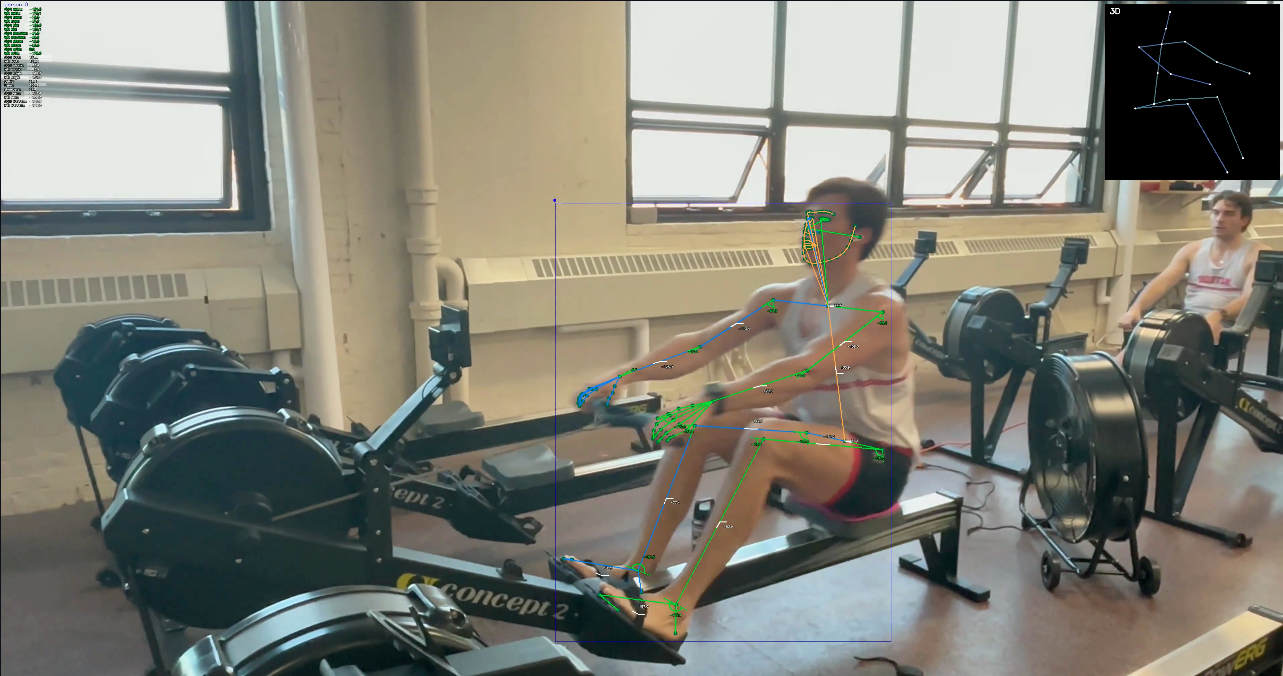
\includegraphics[width=\linewidth]{erg-sports2d.png}
    \caption{Sports2D pose overlay on ergometer video.}
    \label{fig:sports2d-erg}
  \end{subfigure}
  \hfill
  \begin{subfigure}{0.48\linewidth}
    \centering
    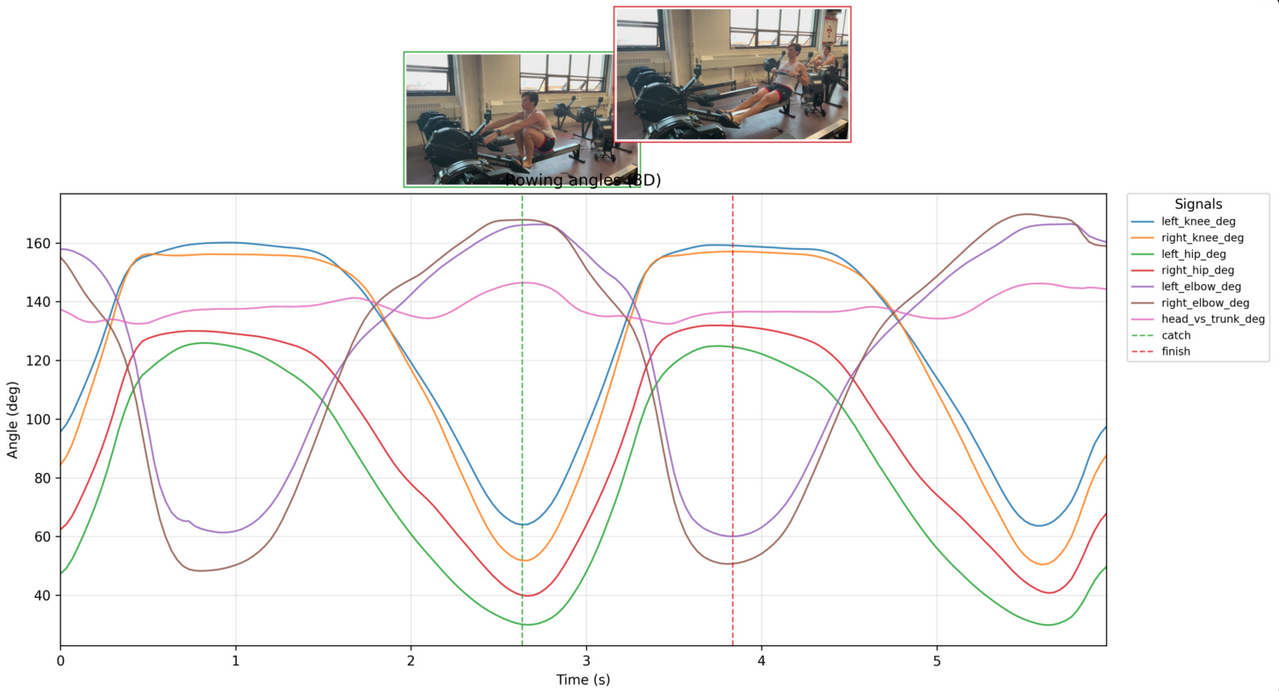
\includegraphics[width=\linewidth]{graph-sports2d.png}
    \caption{Smooth angle traces from the pose pipeline.}
    \label{fig:sports2d-graph}
  \end{subfigure}
  \caption{Pose extraction and kinematic trace generation provide the video-side input to the force-curve alignment pipeline.}
  \label{fig:pose}
\end{figure}

\subsection{Pose and Kinematic Feature Extraction}
Video processing begins with Sports2D pose extraction. The pipeline computes keypoint trajectories and joint angles for rowing-relevant landmarks, including knees, hips, elbows, trunk orientation, spine flexion, and head-trunk angle. MotionBERT lifting is used to improve temporal consistency and support human-motion representation beyond raw image-plane keypoints.

The project initially explored direct MMPose/RTMPose-style two-dimensional extraction, stabilization, cropping, and explicit person tracking. Those experiments showed acceptable results in single-athlete views but degraded under occlusion, oblique camera angles, and multi-athlete identity switching. The Sports2D-first path was adopted because it produced smoother trajectories and better practical iteration speed in ergometer footage.

\subsection{Stroke Progress and Event Detection}
The video-side stroke signal is built from a handle proxy and a machine-reference proxy. The handle proxy is the midpoint of the hand or wrist keypoints, and the machine reference is tracked in the same image sequence. Their relative displacement along the drive axis defines a video-derived progress signal. This signal supports both event detection and reparameterization from time \(t\) to normalized drive progress \(s\).

Catch and finish detection are critical because RP3 force is defined only over the drive. Early versions used the position maximum as the finish, but this overextended the drive: the handle can keep moving after meaningful force production ends. The implemented detector therefore supports velocity-threshold and velocity-calibrated modes. In RP3-supervised runs, a two-pass calibration minimizes video-vs-RP3 drive-duration error by selecting catch and finish velocity fractions. In the calibrated 20-stroke local run, the selected parameters were catch velocity fraction \(0.43\), finish velocity fraction \(0.74\), and a \SI{0.04}{s} smoothing window.

\begin{figure}[t]
  \centering
  \begin{subfigure}{0.48\linewidth}
    \centering
    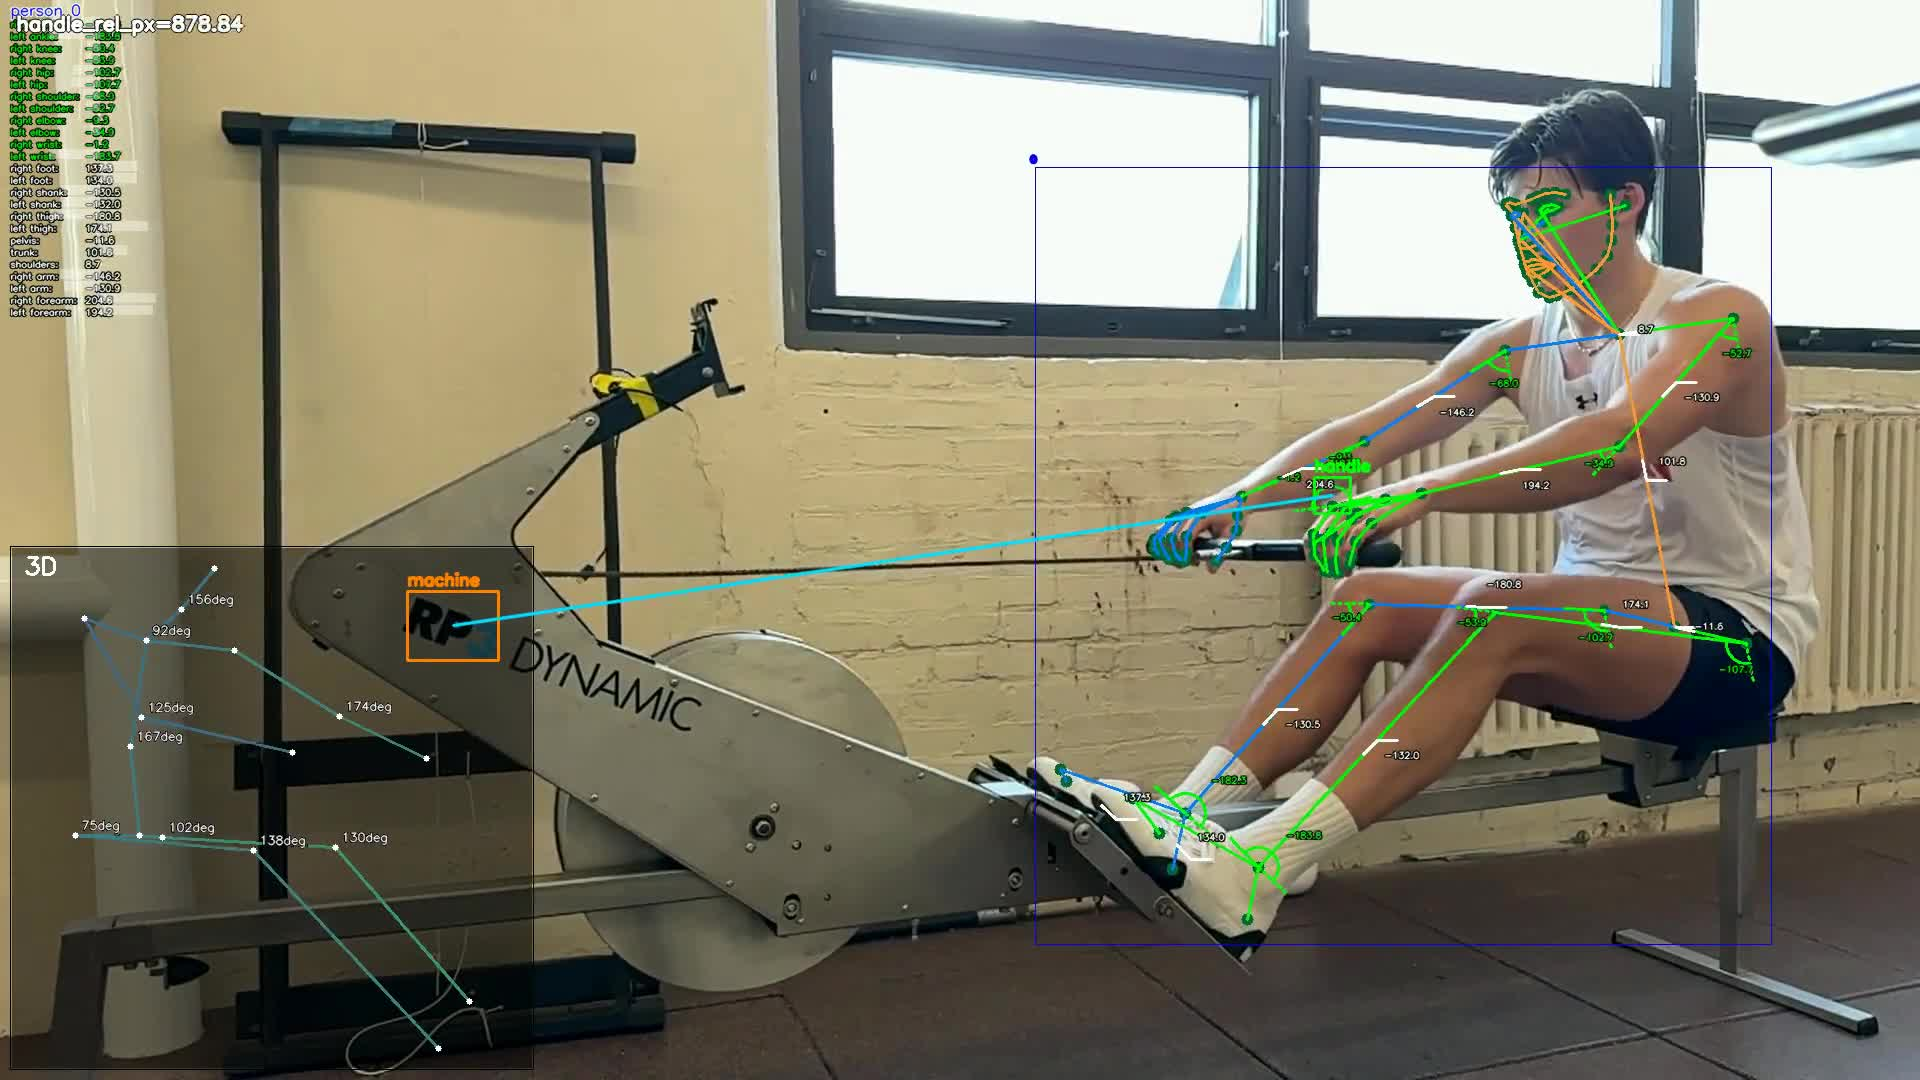
\includegraphics[width=\linewidth]{tracked-handle.jpg}
    \caption{Handle proxy and machine reference tracking.}
    \label{fig:handle}
  \end{subfigure}
  \hfill
  \begin{subfigure}{0.48\linewidth}
    \centering
    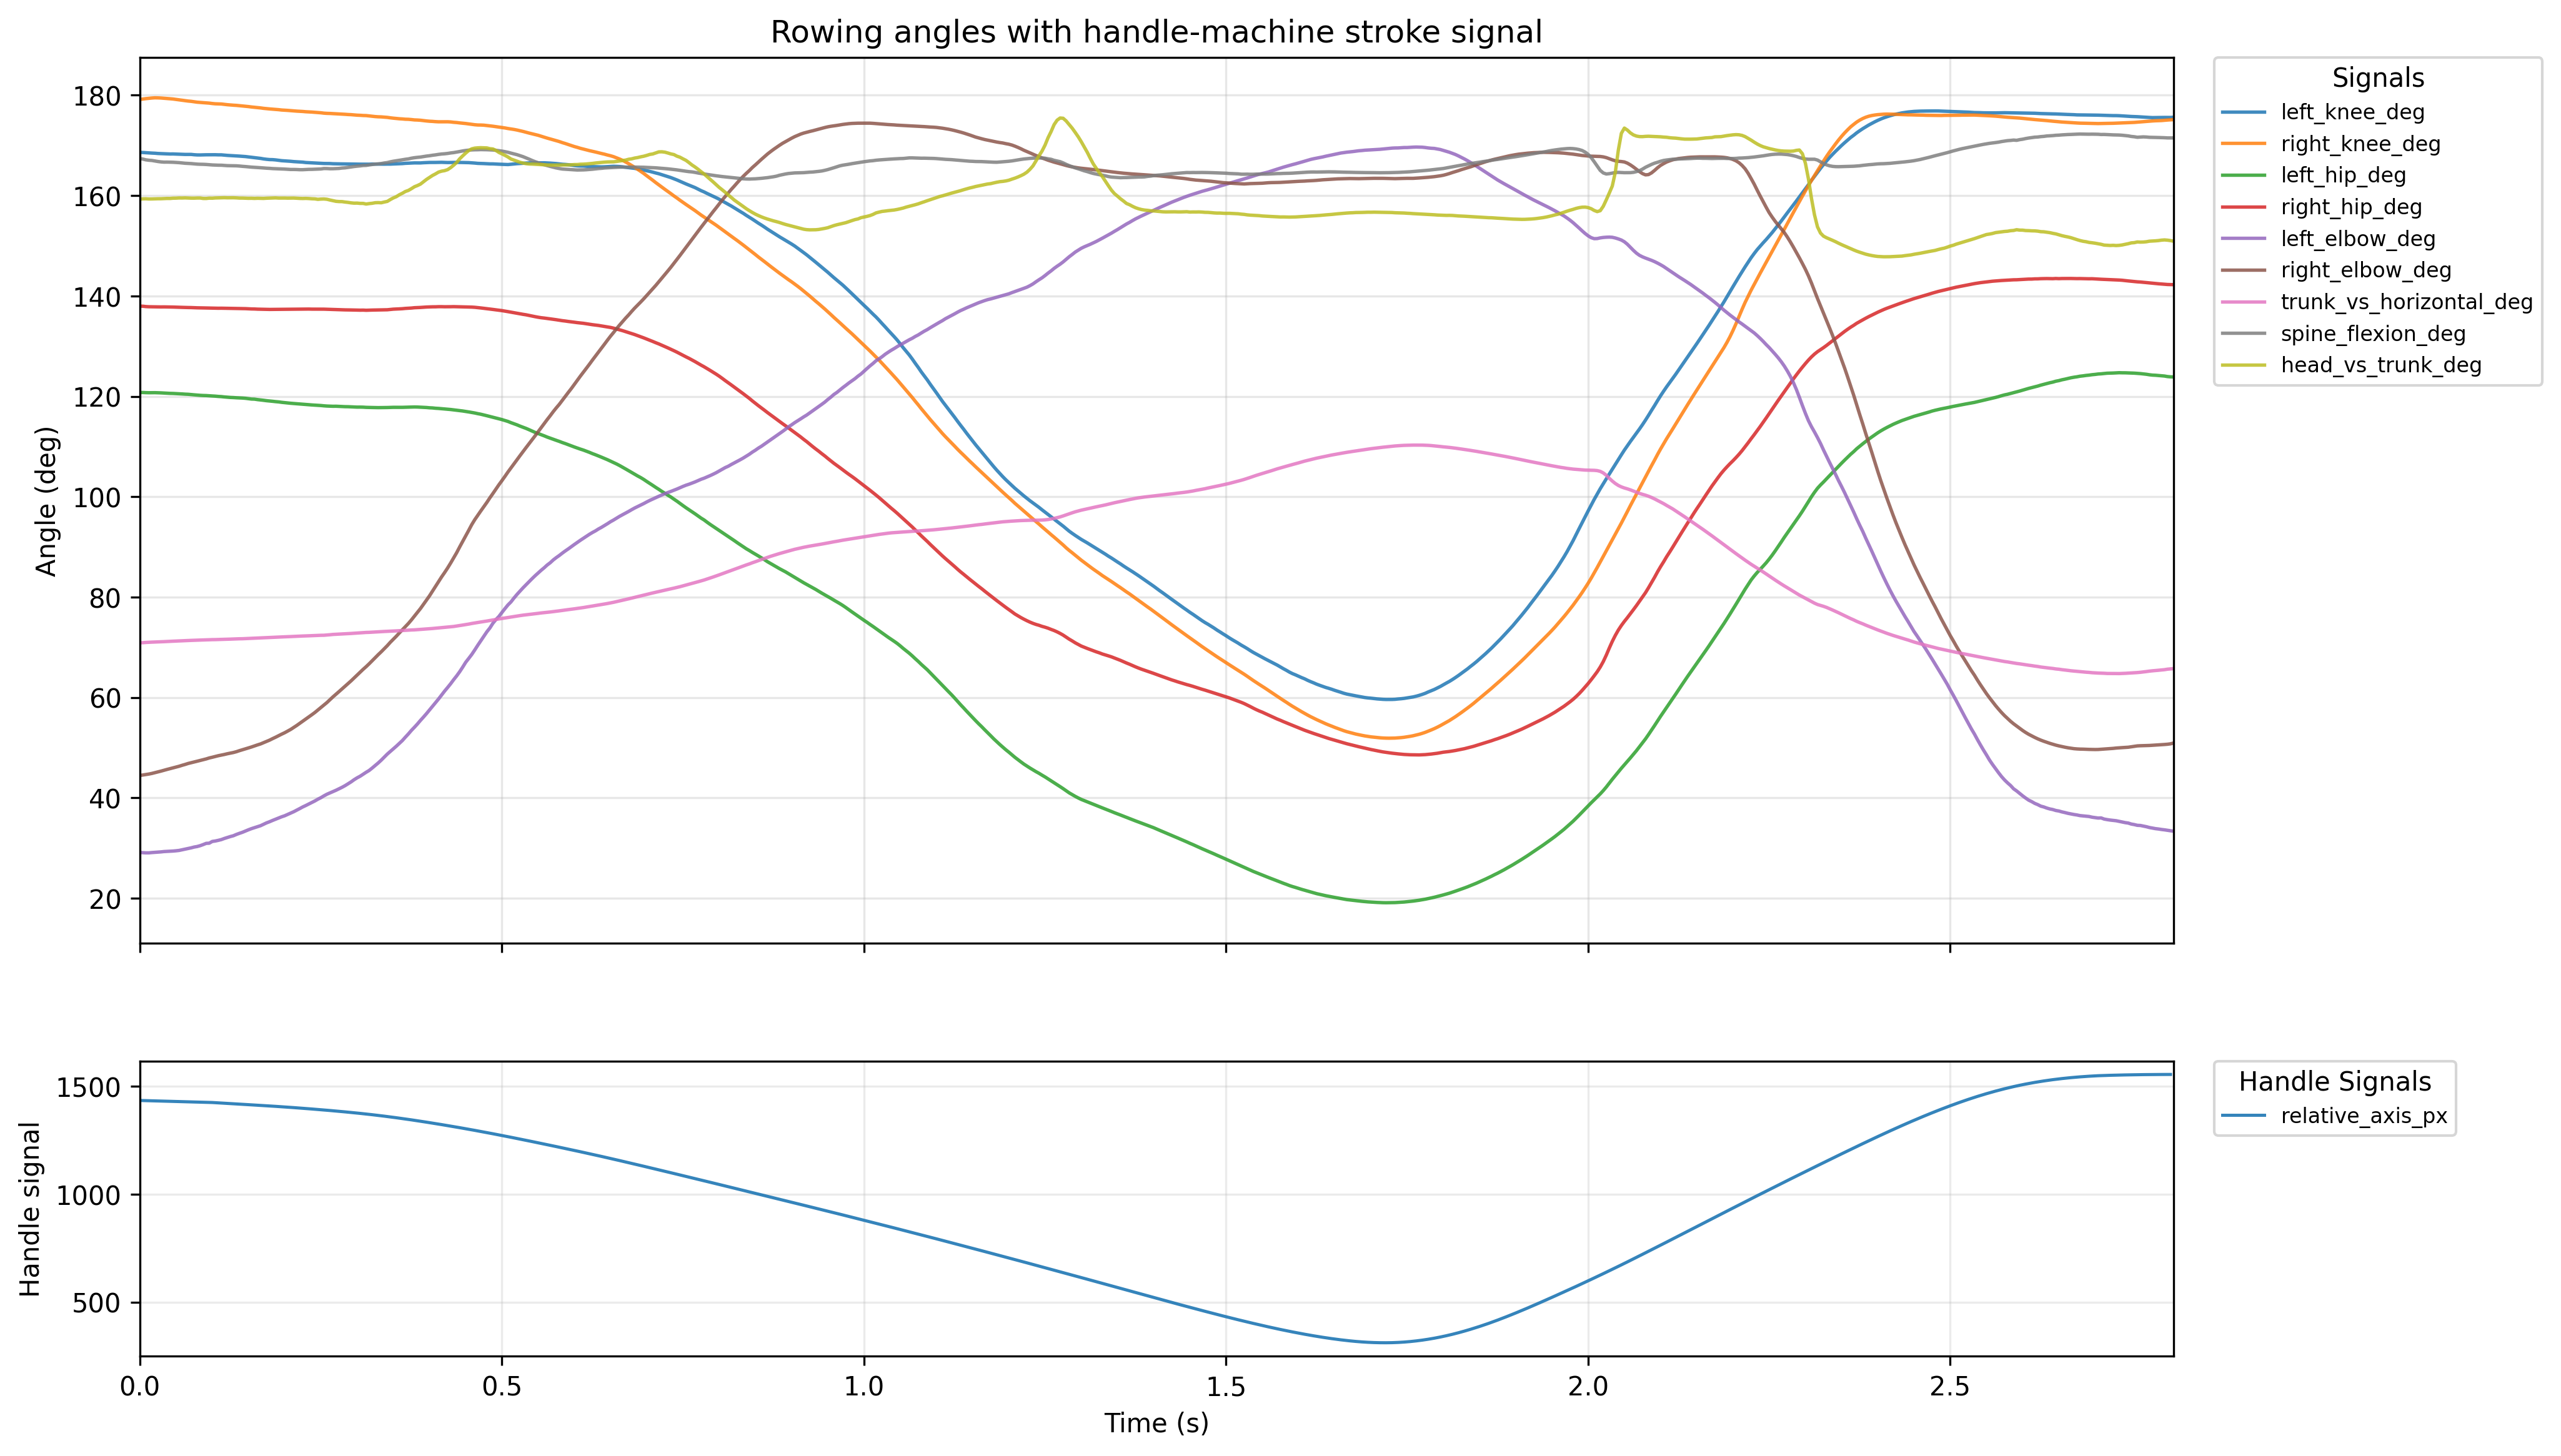
\includegraphics[width=\linewidth]{angles_h36m_with_stroke_plot.png}
    \caption{Kinematic traces with inferred stroke progress.}
    \label{fig:progress}
  \end{subfigure}
  \caption{The current system estimates drive progress from video rather than from a direct machine synchronization channel. This is workable for feasibility testing but introduces sensitivity at catch and finish.}
  \label{fig:progress-tracking}
\end{figure}

\subsection{RP3 Force-Curve Cleaning and Domain Interpretation}
RP3 workout exports contain per-stroke force-curve data and summary metrics. The project verified that RP3 curve samples correspond to a fixed \SI{2.2}{cm} distance step rather than uniform time sampling. The evidence is threefold: curve length matches stroke length divided by \SI{2.2}{cm}, peak-force position matches the index of the maximum curve value after distance scaling, and reconstructed curves match the RP3 portal visualization after linear scaling.

For each RP3 stroke, force samples at distances \(d_k\) are converted to normalized progress
\[
  s_k = \frac{d_k}{L},
\]
where \(L\) is the reported stroke length in centimeters. The force values \(Y(s_k)\) then provide the target curve for supervised learning.

\begin{figure}[t]
  \centering
  \begin{subfigure}{0.48\linewidth}
    \centering
    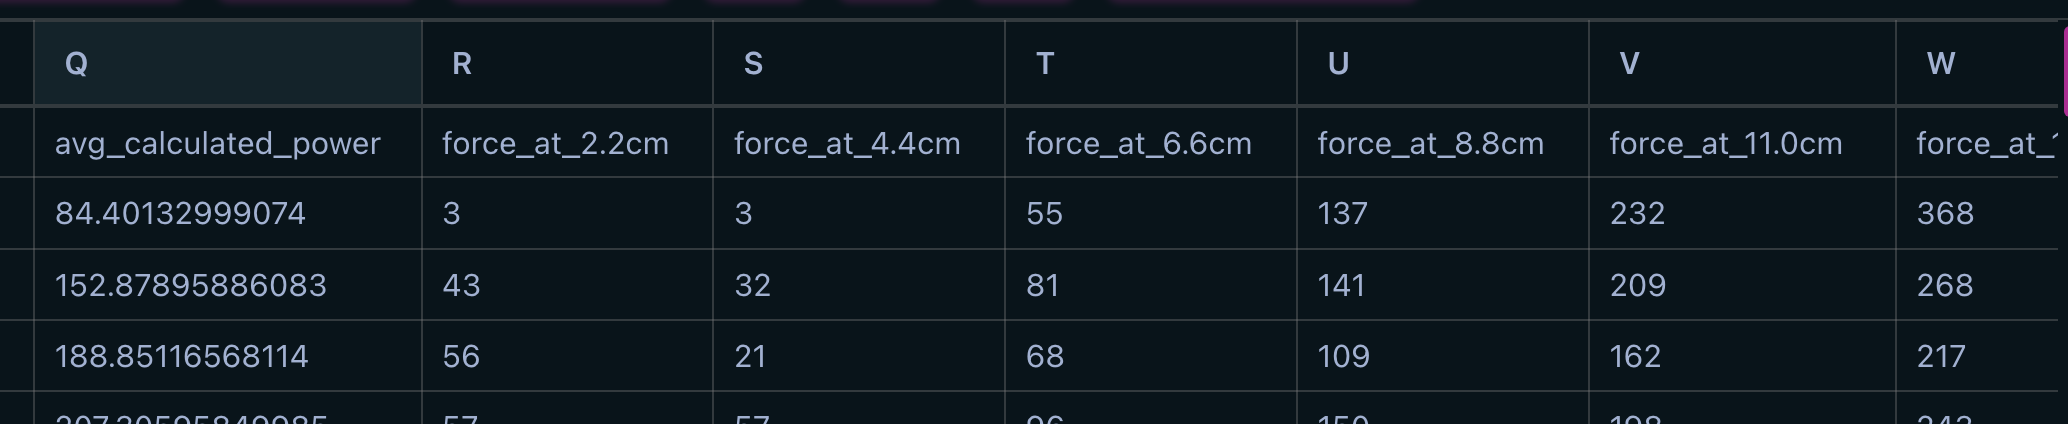
\includegraphics[width=\linewidth]{cleaned-data.png}
    \caption{Cleaned RP3 force data.}
    \label{fig:rp3-cleaned}
  \end{subfigure}
  \hfill
  \begin{subfigure}{0.48\linewidth}
    \centering
    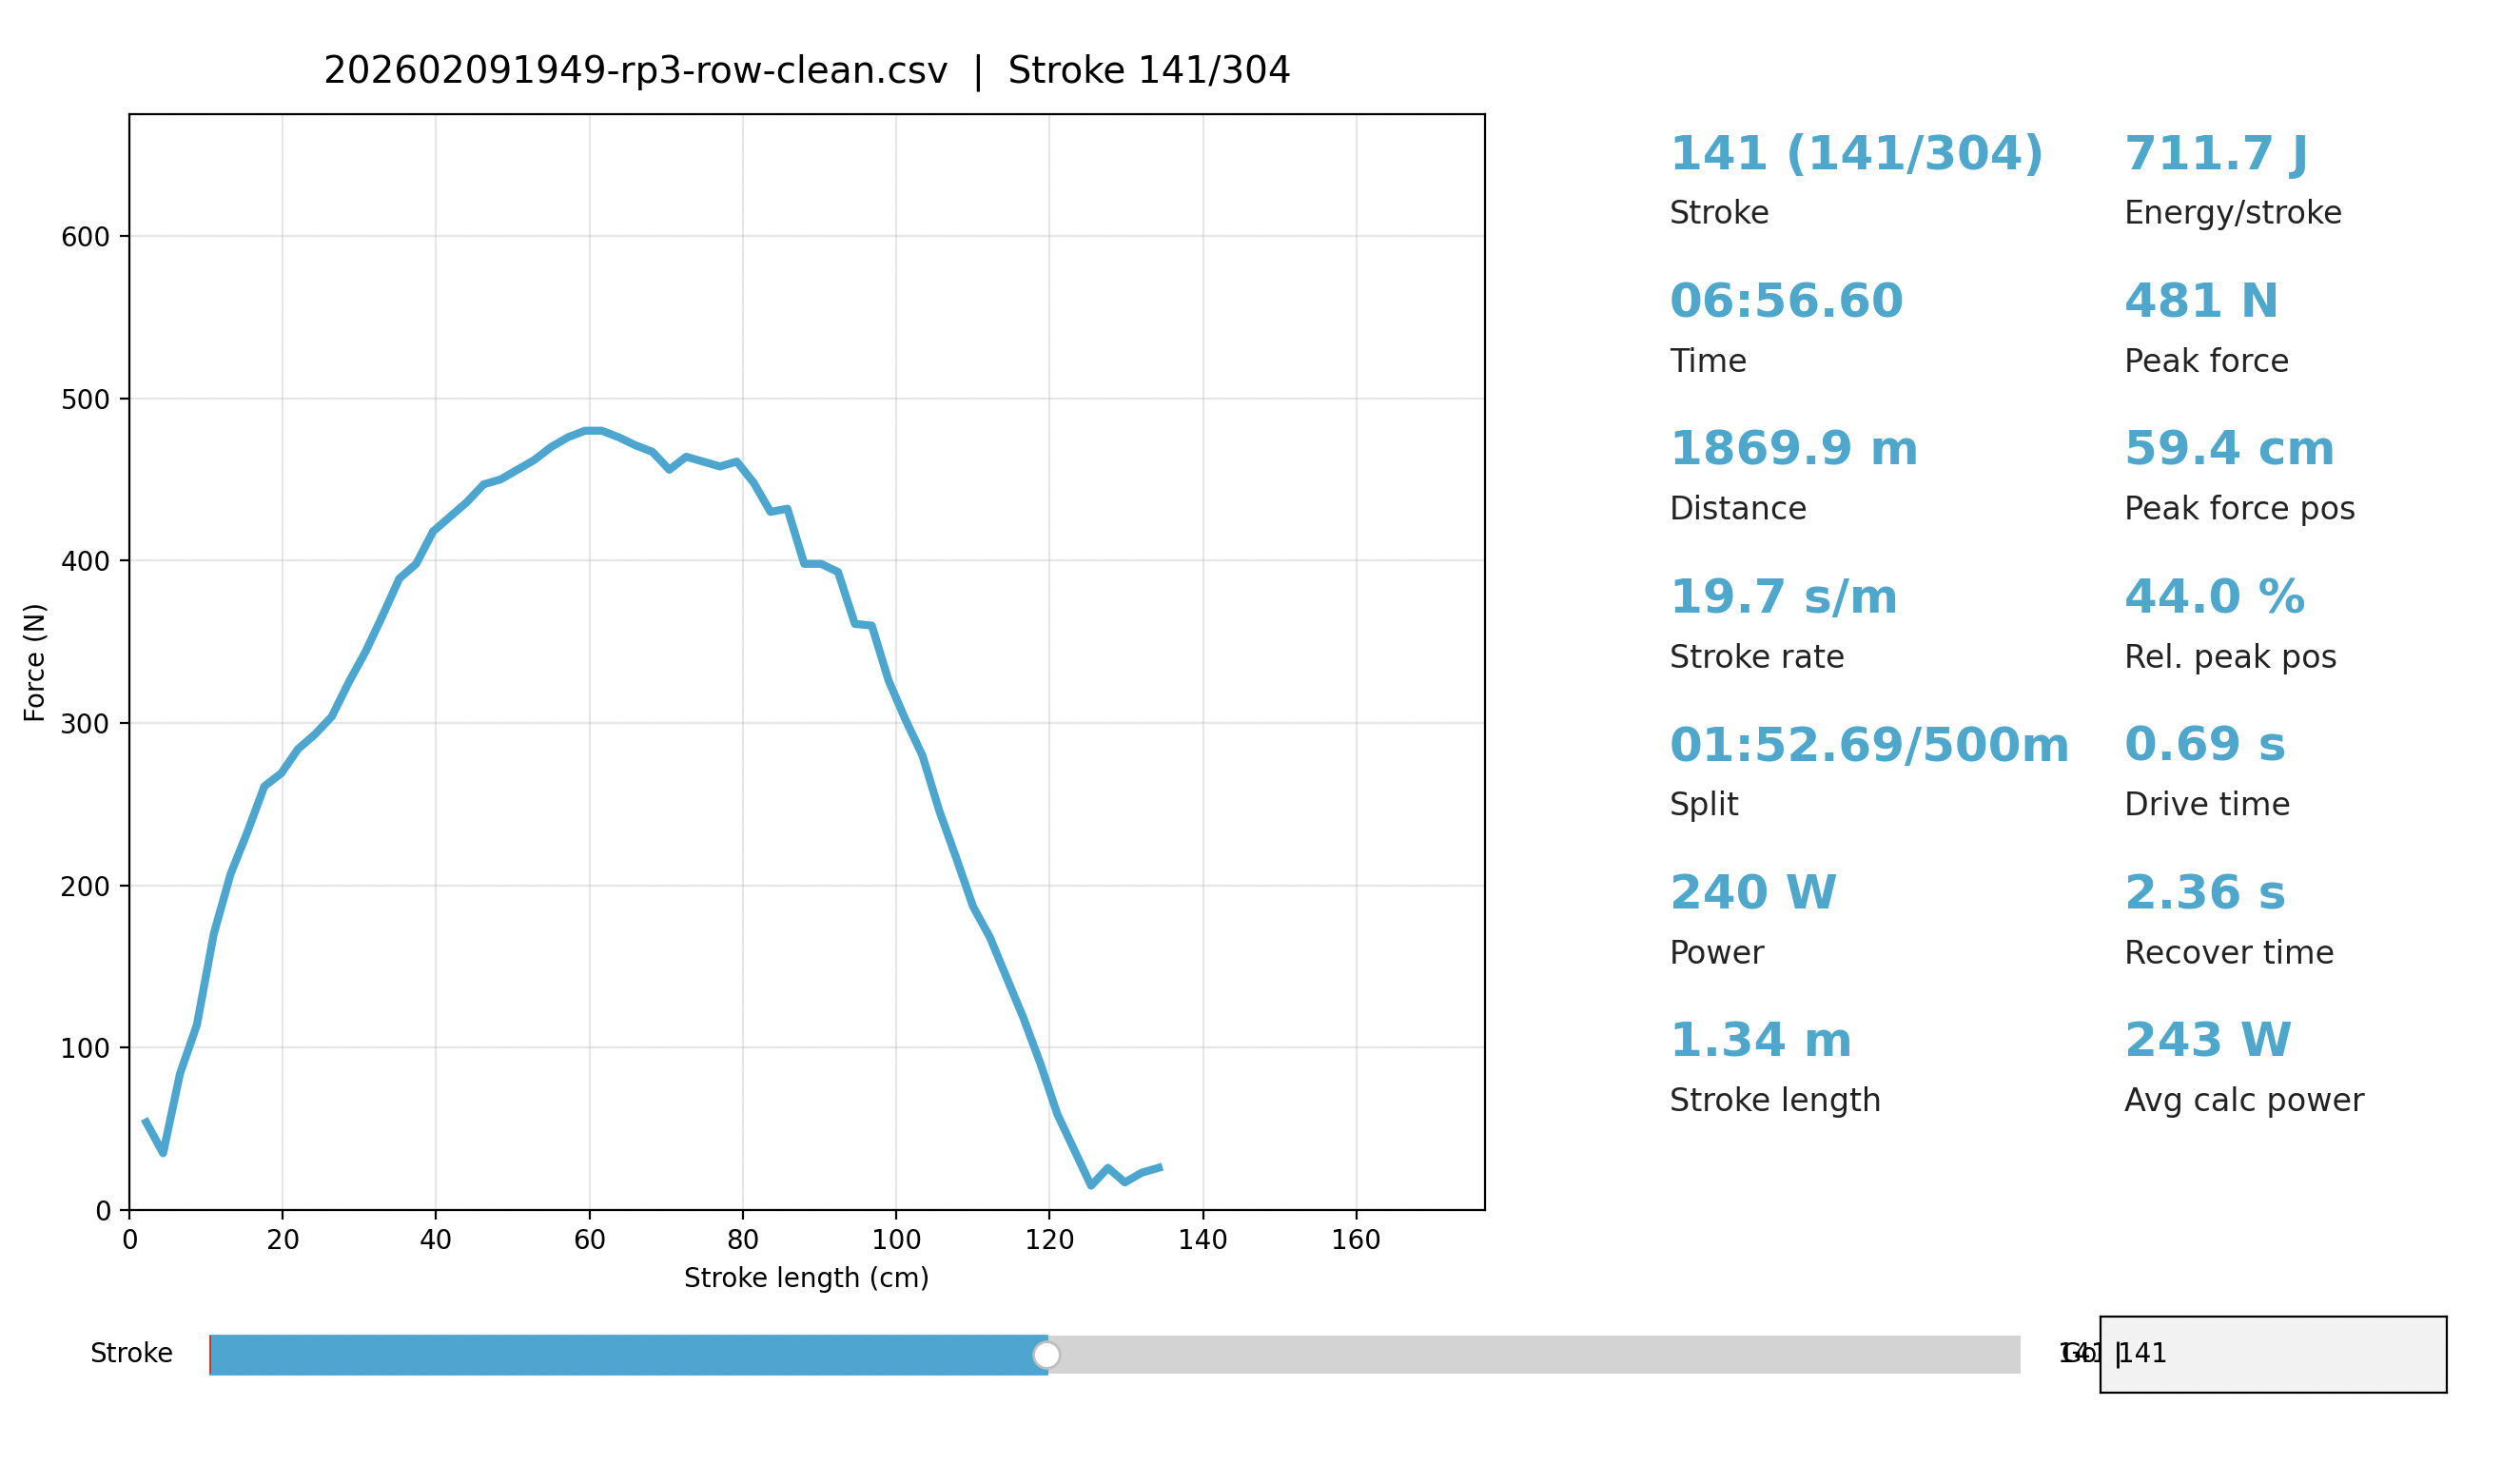
\includegraphics[width=\linewidth]{recreation.png}
    \caption{Per-stroke RP3 curve recreation.}
    \label{fig:rp3-recreation}
  \end{subfigure}
  \caption{RP3 force exports are interpreted as distance-domain curves sampled every \SI{2.2}{cm}, enabling alignment to video-derived normalized drive progress.}
  \label{fig:rp3}
\end{figure}

\subsection{Feature Contract and Alignment}
Each supervised sample is one matched stroke. Inputs are kinematic curves and support features over \(s \in [0,1]\). The canonical feature contract includes active-side knee, hip, and elbow angles; trunk angle; spine flexion; head-trunk angle; progress-domain derivatives; and handle velocity/acceleration. Left/right source columns are canonicalized through an \texttt{active\_side} setting, and trunk orientation is mirror-normalized when camera geometry requires it.

Video kinematics are interpolated onto the RP3 force-bin progress values. First derivatives are computed by differentiating in time and applying the chain rule:
\[
  \frac{d\theta}{ds}
    =
  \frac{d\theta/dt}{ds/dt + \epsilon}.
\]
This avoids differentiating directly on irregular progress samples and reduces derivative instability. Optional second derivatives are supported but disabled by default because they amplify noise unless validated by ablation.

\subsection{Quality Control}
Quality-control flags are preserved rather than silently dropping suspicious strokes. The implemented gates include sparse tracking, non-physiological angular velocity, handle-progress stalls, nonmonotonic progress repairs, weak detection confidence, implausible duration, alignment drift, and video/RP3 rate mismatch. A continuous \texttt{stroke\_quality\_score} combines these signals for downstream filtering and inference confidence.

\subsection{Dataset and Modeling Artifacts}
The dataset builder pivots long-format segment CSVs into one record per stroke and creates two target representations. The first preserves native RP3 bins in padded arrays with masks. The second resamples force and kinematic features to a fixed 64-point grid over normalized drive progress. PCA is fitted to peak-normalized force curves, and scalar summaries of kinematics are added to \texttt{strokes.csv}.

The modeling code is staged. Stage 0 measures a reproducibility floor and metadata-only baselines using stroke rate, stroke length, and drive time. Stage A fits interpretable models from scalar kinematic summaries to PCA force-curve coefficients. Stage B defines sequence models, including temporal convolutional and transformer architectures, for direct curve prediction. Evaluation helpers report RMSE, MAE, curve correlation, peak-force error, peak-position error, impulse error, early/mid/late-drive MAE, and alignment integrity. The code explicitly labels single-athlete or within-athlete splits as provisional and reserves generalization claims for athlete-held-out evaluation.

\section{Results}
\subsection{Local Data Availability}
The repository contains two matched segment exports and one session registry. The registry lists two planned athletes, \texttt{giacomo-cappelletto} and \texttt{mason-laundry}, but the matched segment artifacts found locally are both Giacomo runs. Therefore, the available results support only pipeline feasibility and alignment analysis, not cross-athlete prediction.

\begin{table}[t]
  \centering
  \caption{Available local matched artifacts. Values are derived from \texttt{rp3\_match\_summary.json}, \texttt{drive\_events\_summary.json}, and \texttt{rp3\_pose\_force\_matched\_segments.csv}.}
  \label{tab:artifacts}
  \sisetup{round-mode=places,round-precision=3}
  \small
  \begin{tabularx}{\linewidth}{Xrrrrr}
    \toprule
    Run & Strokes & Rows & FPS & Length (cm) & Peak (N) \\
    \midrule
    \texttt{giacomo-20strokes} & 20 & 1,203 & 120.003 & 132.330 & 497.900 \\
    \texttt{bad-giacomo-10m} & 208 & 12,629 & 120.048 & 133.576 & 503.452 \\
    \bottomrule
  \end{tabularx}
\end{table}

Table~\ref{tab:artifacts} shows that the pipeline can produce substantial aligned training rows from a single ergometer session. However, force-curve prediction models require independent variation across athletes, sessions, camera geometry, intensity, and stroke style. The local evidence does not provide that variation.

\subsection{Stroke Matching and Timing Integrity}
The calibrated 20-stroke run achieved close video/RP3 drive-duration agreement. Mean absolute drive-duration error was \SI{0.011}{s}, mean absolute interval error was \SI{0.064}{s}, and mean absolute cumulative catch error was \SI{0.208}{s}. This demonstrates that the velocity-calibrated event detector can align short runs accurately when drift is limited.

The older 208-stroke run illustrates the dominant failure mode. It exported 208 strokes and achieved mean absolute drive-duration error of \SI{0.032}{s}, but mean absolute cumulative catch error reached \SI{2.360}{s}. Thus, individual drive windows can appear plausible while cumulative alignment drifts enough to corrupt stroke labels across a longer piece.

\begin{table}[t]
  \centering
  \caption{Alignment diagnostics from local matched runs. Lower values indicate better video/RP3 agreement.}
  \label{tab:alignment}
  \sisetup{round-mode=places,round-precision=3}
  \small
  \begin{tabularx}{\linewidth}{Xrrrr}
    \toprule
    Run & Drive MAE (s) & Interval MAE (s) & Cum. catch MAE (s) & Strokes \\
    \midrule
    \texttt{giacomo-20strokes} & 0.011 & 0.064 & 0.208 & 20 \\
    \texttt{bad-giacomo-10m} & 0.032 & 0.022 & 2.360 & 208 \\
    \bottomrule
  \end{tabularx}
\end{table}

\begin{figure}[t]
  \centering
  \begin{subfigure}{0.48\linewidth}
    \centering
    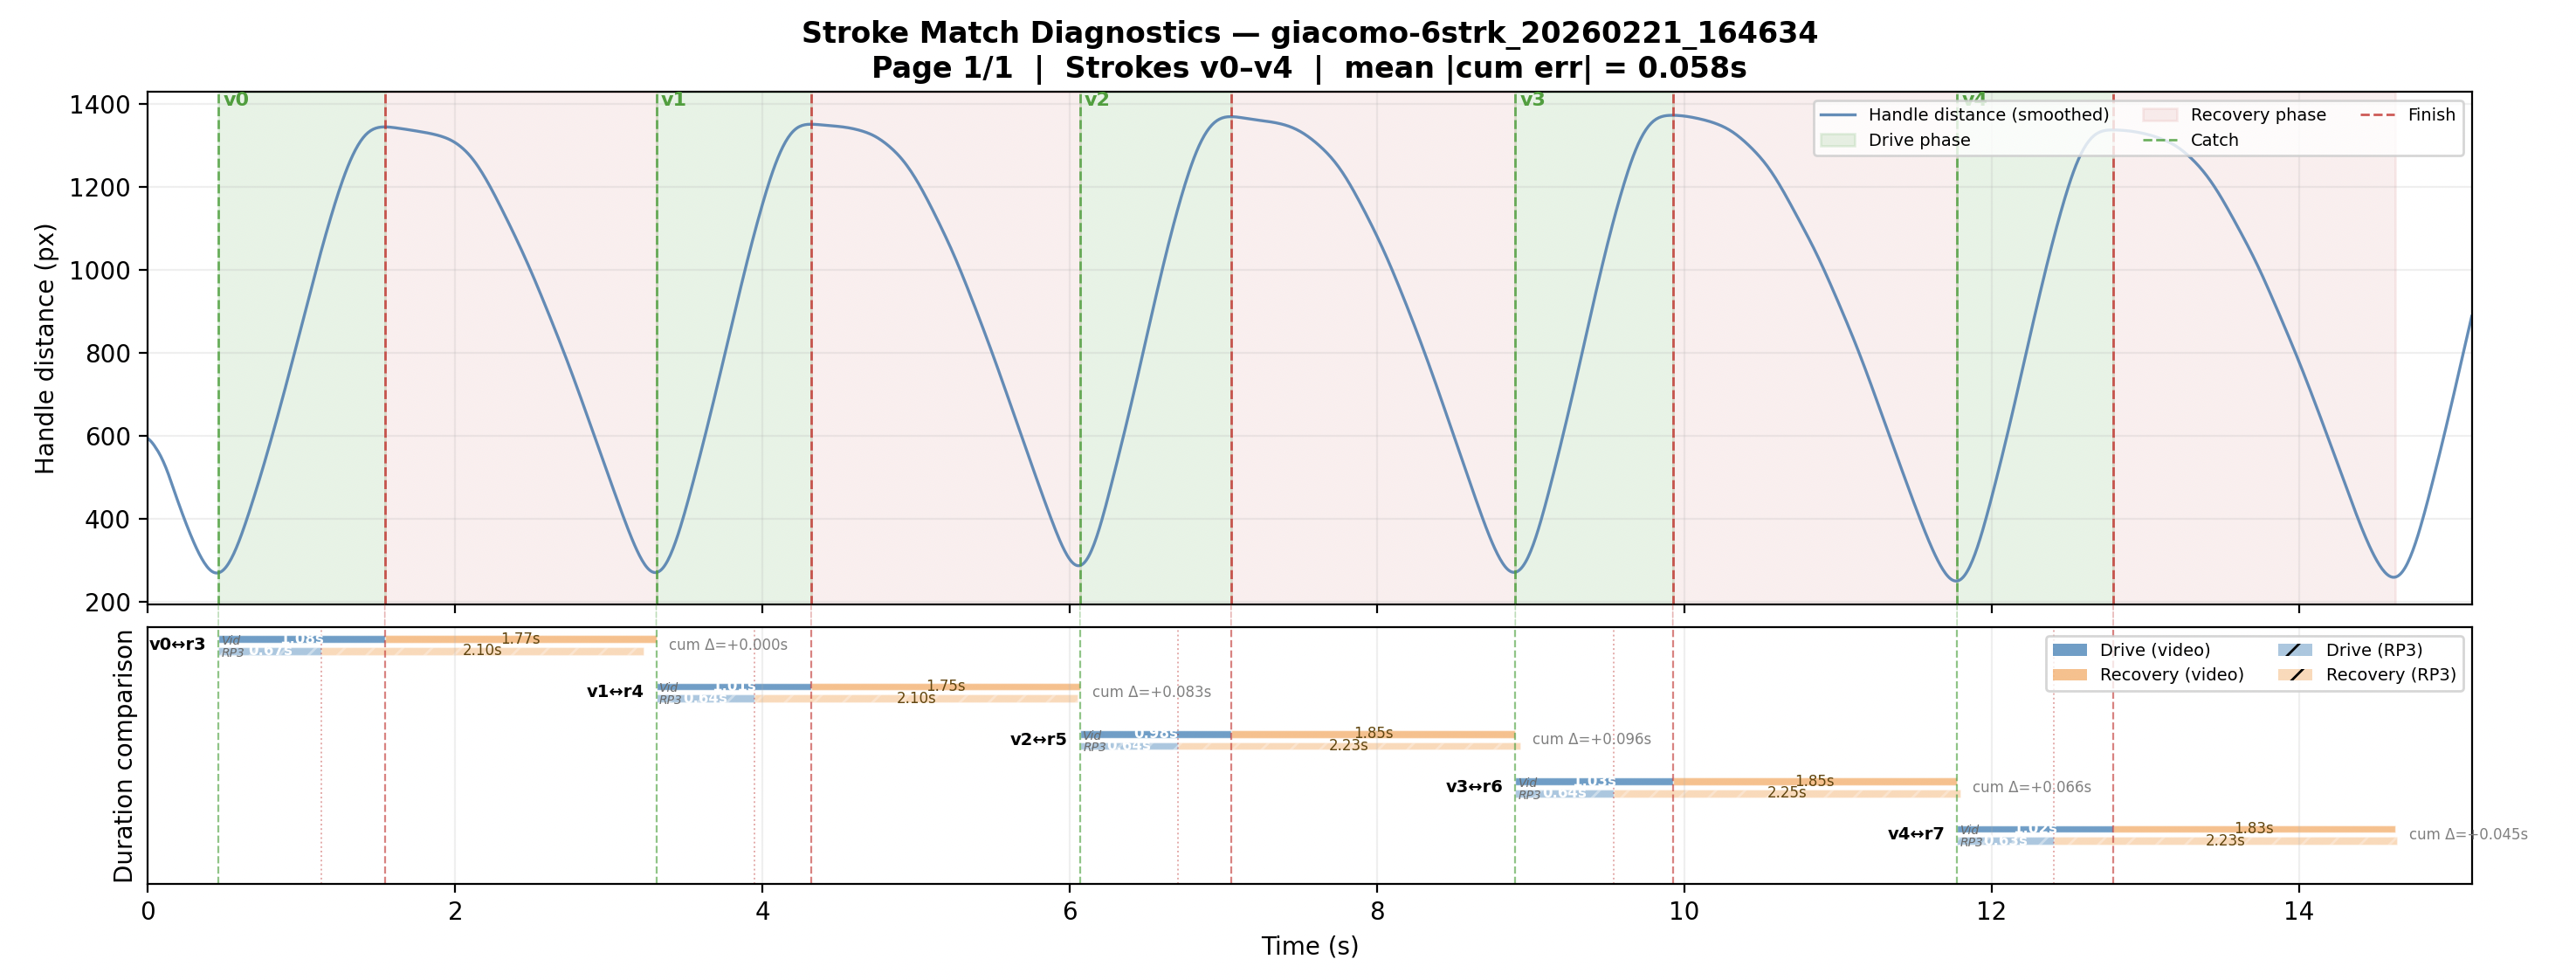
\includegraphics[width=\linewidth]{stroke-matching.png}
    \caption{Stroke-matching diagnostics showing drift and mismatch.}
    \label{fig:stroke-matching}
  \end{subfigure}
  \hfill
  \begin{subfigure}{0.48\linewidth}
    \centering
    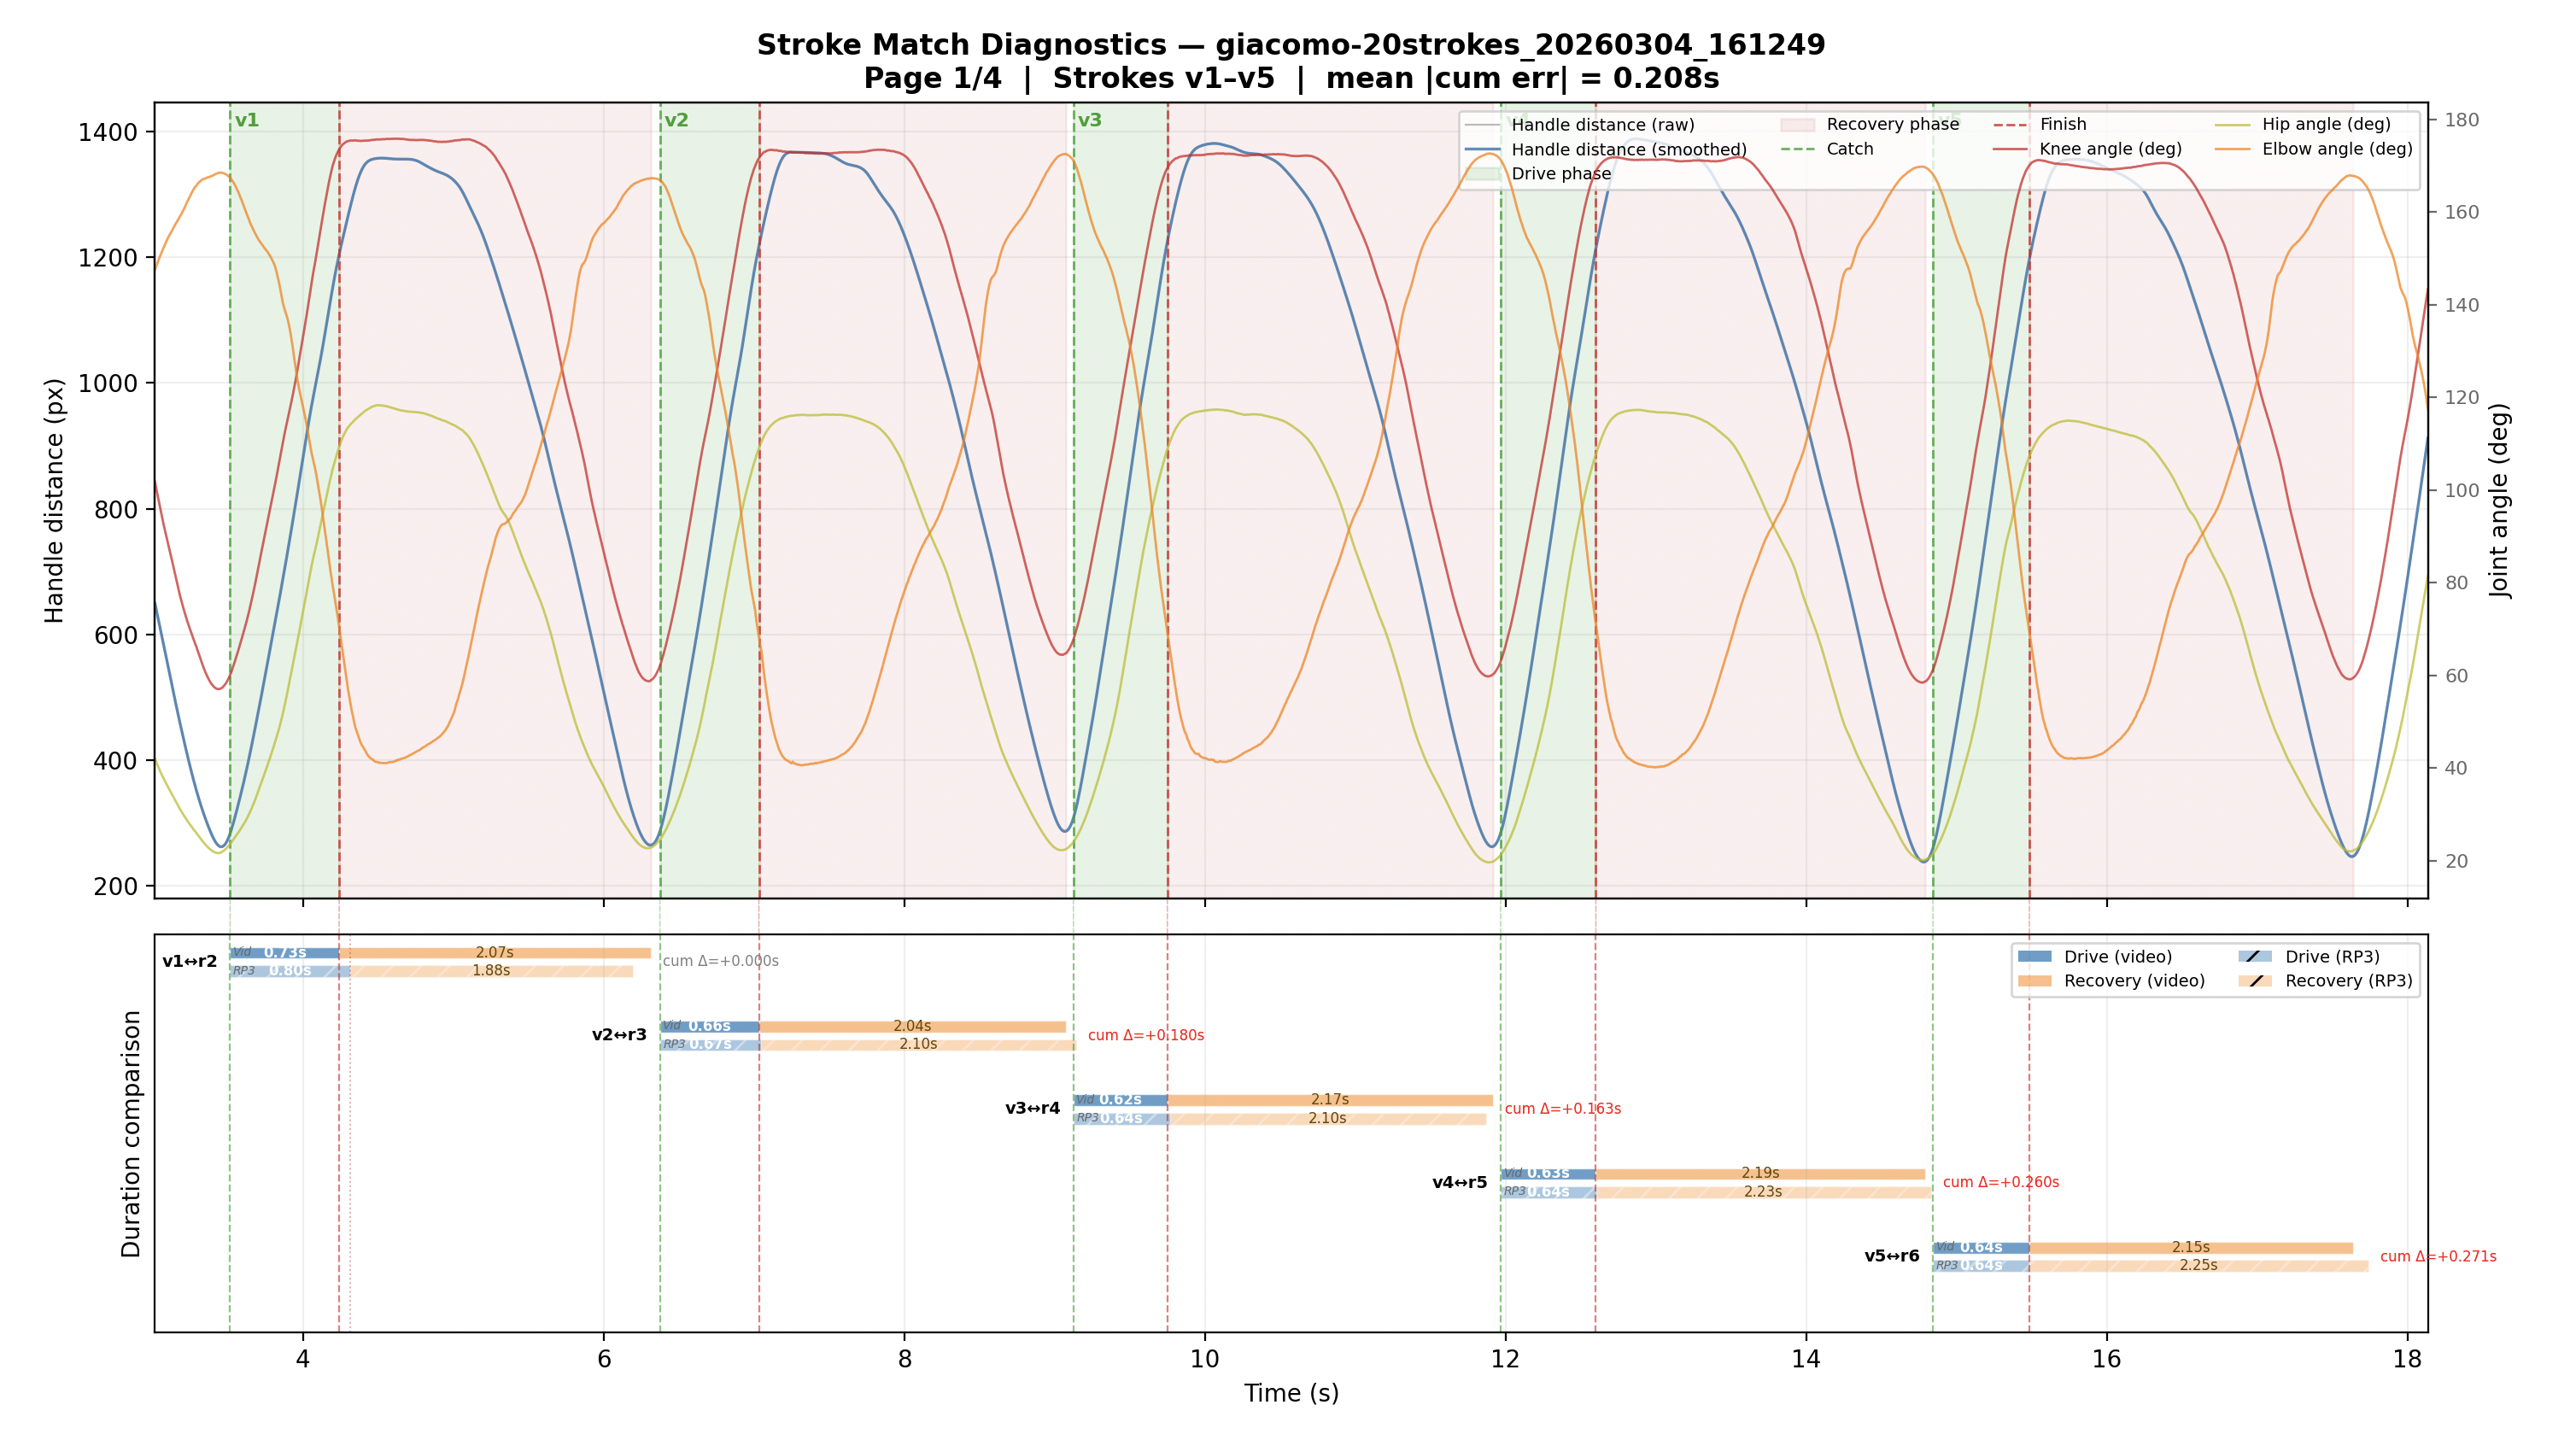
\includegraphics[width=\linewidth]{matching-with-angles.png}
    \caption{Matching diagnostics interpreted against angle traces.}
    \label{fig:matching-angles}
  \end{subfigure}
  \caption{Stroke matching remains the highest-risk stage because small event-timing errors occur where force-curve labels are most sensitive.}
  \label{fig:matching}
\end{figure}

\subsection{Implications for Prediction}
No local athlete-held-out modeling artifact was found. Under the repository's own evaluation regime, this means that any model result from the available data would be provisional. Training and testing on temporally adjacent strokes from the same athlete would primarily measure interpolation within one movement pattern, not generalization to new athletes.

The available evidence also indicates why a small stroke count is insufficient. A 20-stroke run can validate a calibration mechanism, but it cannot span enough variability in fatigue, rate, intensity, morphology, technique, or camera geometry. A 208-stroke run provides more rows but still comes from a single athlete and shows cumulative drift. More rows from the same correlated session do not substitute for independent athlete diversity.

\section{Discussion}
The project demonstrates a technically coherent route from monocular rowing video to aligned force-curve training samples. The strongest outcome is the construction of a reproducible feature and target contract: video-derived biomechanics can be represented in the same normalized drive-progress domain as RP3 force curves, exported as matched segments, and converted into model-ready artifacts.

The main weakness is not the absence of a model architecture. The repository already contains reasonable Stage 0, Stage A, and Stage B modeling paths. The limiting factor is label quality and data diversity. Catch timing, finish timing, and drive progress are inferred from video proxies. These approximations are most consequential at precisely the phases where force curves are most sensitive: force onset near the catch, peak-force development through the drive, and force drop-off near the finish. The 208-stroke run shows that a label stream can drift even when per-stroke drive durations look plausible.

For this reason, future accuracy improvements should prioritize synchronized measurement before model complexity. A direct connection to the ergometer or rowing machine telemetry stream would provide shared timestamps, exact drive boundaries, and machine-native stroke progress. That connection would reduce the need to infer the most sensitive labels from approximate video events. Once synchronized data are available, the existing feature contract, QC gates, and evaluation helpers can be used to test whether biomechanics adds predictive value beyond metadata-only baselines.

\section{Limitations}
The present study has four major limitations. First, matched local artifacts are single-athlete despite the registry listing two planned athletes. This prevents athlete-held-out evaluation. Second, the matched runs are not balanced across camera viewpoint, rowing intensity, fatigue state, or athlete morphology. Third, the current video-derived progress signal is approximate and can accumulate drift. Fourth, no compiled model result in the repository establishes that the Stage A or Stage B predictors improve on metadata-only baselines under a valid generalization split.

These limitations are substantial, but they are informative rather than incidental. They define the next experimental requirement: collect synchronized, diverse, athlete-balanced video and telemetry data before making predictive claims.

\section{Conclusion}
This project implements a full video-to-biomechanics-to-force data pipeline for rowing. It can extract pose, infer stroke events, clean RP3 force curves, align video kinematics to force bins, export matched segments, and create model-ready datasets. Real local artifacts show feasibility for short calibrated runs and expose drift risk in longer runs. However, the current data are not sufficient for reliable prediction of new athletes. Achieving the desired accuracy will require more strokes, broader athlete diversity, balanced recording conditions, and direct synchronized telemetry from the rowing machine.

\section*{Data and Code Availability}
The manuscript is based on the local repository \texttt{rowing-video-analysis}. Numeric results reported here are traceable to \texttt{session\_registry.csv} and the two local inference artifact directories for \texttt{giacomo-20strokes} and \texttt{bad-giacomo-10m}. The two dirty/untracked documentation files present during manuscript preparation were not modified.

\bibliographystyle{plainnat}
\bibliography{paper/references}

\end{document}
